% Chapter Background

\chapter{Background: SCION Future Internet Architecture} % Main chapter title

\label{background} % For referencing the chapter elsewhere, use \ref{background}
% Leading paragraph is missing
% Move 2.11 here
SCION \cite{PeSzReCh2017, scion_cacm_2017} and APNA both are security oriented architecture which leads to an interesting question: Can we combine two security-oriented architectures to benefit from the advantages of the both architecture? We try to address this question by integrating APNA with SCION. In addition to that there are other compelling reasons for the integration:
\begin{itemize}
    \item SCION clearly distinguish between inter-domain and intra-domain routing and its very easy to replace existing IP based intra-domain routing protocol to APNA's Ephemeral Identifiers.
    \item SCION also provides various AS level services such as certificate server to manage all AS level certificates which is ideal for managing all the keys used by different services inside APNA Management Service.
    \item SCION as framework also provides a mechanisms to create new AS level data plane services which could be used to process APNA packet.
    \item SCION has an existing deployed testbed (i.e., SCIONLab) which is ideal for experimentation purpose.
\end{itemize}

Thus it would be a good idea to get a better understanding about the internals of SCION discussing the integration of the two architectures. This chapter provides an overview about SCION and its internal design decisions: Section \ref{sec:about_scion} describes a higher level overview of SCION. Section \ref{sec:isd}, \ref{sec:as} describes how SCION divides the data-plane into logical groups. Section \ref{path_res} provide details about path resolution inside SCION. Section \ref{addr_scheme} talks about the addressing scheme used inside SCION. Section \ref{serv_infra} discusses about the service infrastructure inside SCION and how those services coordinate together to provide all the security guarantees promised by SCION. Section \ref{sec:scion_impl} discuss about implementation details specific to SCION and provides an example to write a basic client-server application using SCION.

\section{What is SCION?} \label{sec:about_scion}
SCION is the new clean state internet architecture designed to provide explicit route control, failure isolation, and explicit trust information for end-to-end communication. SCION organizes existing ASes into groups of independent routing planes, called isolation domains, which interconnect to provide global connectivity. Isolation domains provide natural isolation of routing failures and misconfigurations, give endpoints strong control for both inbound and outbound traffic, provide meaningful and enforceable trust, and enable scalable routing updates with high path diversity. As a result, the SCION architecture provides strong resilience and security properties as an intrinsic consequence of its design.

Besides high security, SCION also provides a scalable routing infrastructure, and high efficiency for packet forwarding. As a path-based architecture, SCION end hosts learn about available network path segments, and combine then into end-to-end paths that are carried in packet headers. For the first time endhost have complete flexibility about how their packets are going to traverse on the internet. ISPs and receivers, offering path choice to all the parties: senders, receivers, and ISPs. This approach enables path-aware communication, an emerging trend in networking. These features also enable multi-path communication, which is an important approach for high availability, rapid fail-over in case of network failures, increased end-to-end bandwidth, dynamic traffic optimization, and resilience to DDoS attacks.

% Not needed
% \subsection{Why a clean-slate design? Why can't we patch the current Internet with existing solutions?}
% It is turning into a litany that the internet was not designed to become the network it now is. Indeed some of its original features are seriously compromising the communications’ privacy and security. 

% One of the core issue is the trust needed to route IP packets between various Autonomous Systems (AS), i.e. internet domains managed by a single entity. According to Wikipedia, the number of ASes multiplied tenfold between 1999 and 2014 from 5000 to 47000. Knowing if you can trust an AS to transport your packets is no sinecure. Several models are proposed to address this issue. However none of these is fully satisfactory: either internet players need to agree on a single root of trust to vouch for everybody else (e.g. RPKI for BGPSEC or DNSSEC) in a context of high political division or the trust is delegated to a number of roots of trust, such as TLS PKI which relies on more than a thousand roots of trust and where the certificate is accepted is signed by any of these and which offers little progress to the original situation.

% The Internet was not designed as a high-security network. Security improvements primarily address specific attacks, but do not solve the fundamental problems and often introduce new undesirable consequences (e.g., BGPSEC prevents route hijacking but causes delayed route convergence, and does not support prefix aggregation which contributes to reduce scalability). With a clean-slate design, we can fundamentally improve the security to a level that is unlikely to be achievable through incremental changes.

\section{Isolation Domains (ISD)} \label{sec:isd}
SCION introduces the concept of an \textbf{isolation domains (ISD)}, which is a fundamental building block for achieving the properties of high availability, transparency, scalability and support for heterogeneous trust.

\section{Autonomous System (AS)} \label{sec:as}
An ISD constitutes a logical grouping of autonomous systems (ASes), as depicted in Figure \ref{fig:isd_as}. An ISD is administered by multiple ASes, which form the \textbf{ISD core}. We refer to these as \textbf{core ASes}. An ISD usually also contains multiple regular ASes. The ISD is governed by a policy, called the \textbf{trust root configuration (TRC)}, which is negotiated by the ISD core. The TRC defines the roots of trust that are used to validate bindings between names and public keys or addresses.

\begin{figure}[th!!]
\centering
\noindent
\makebox[\textwidth]{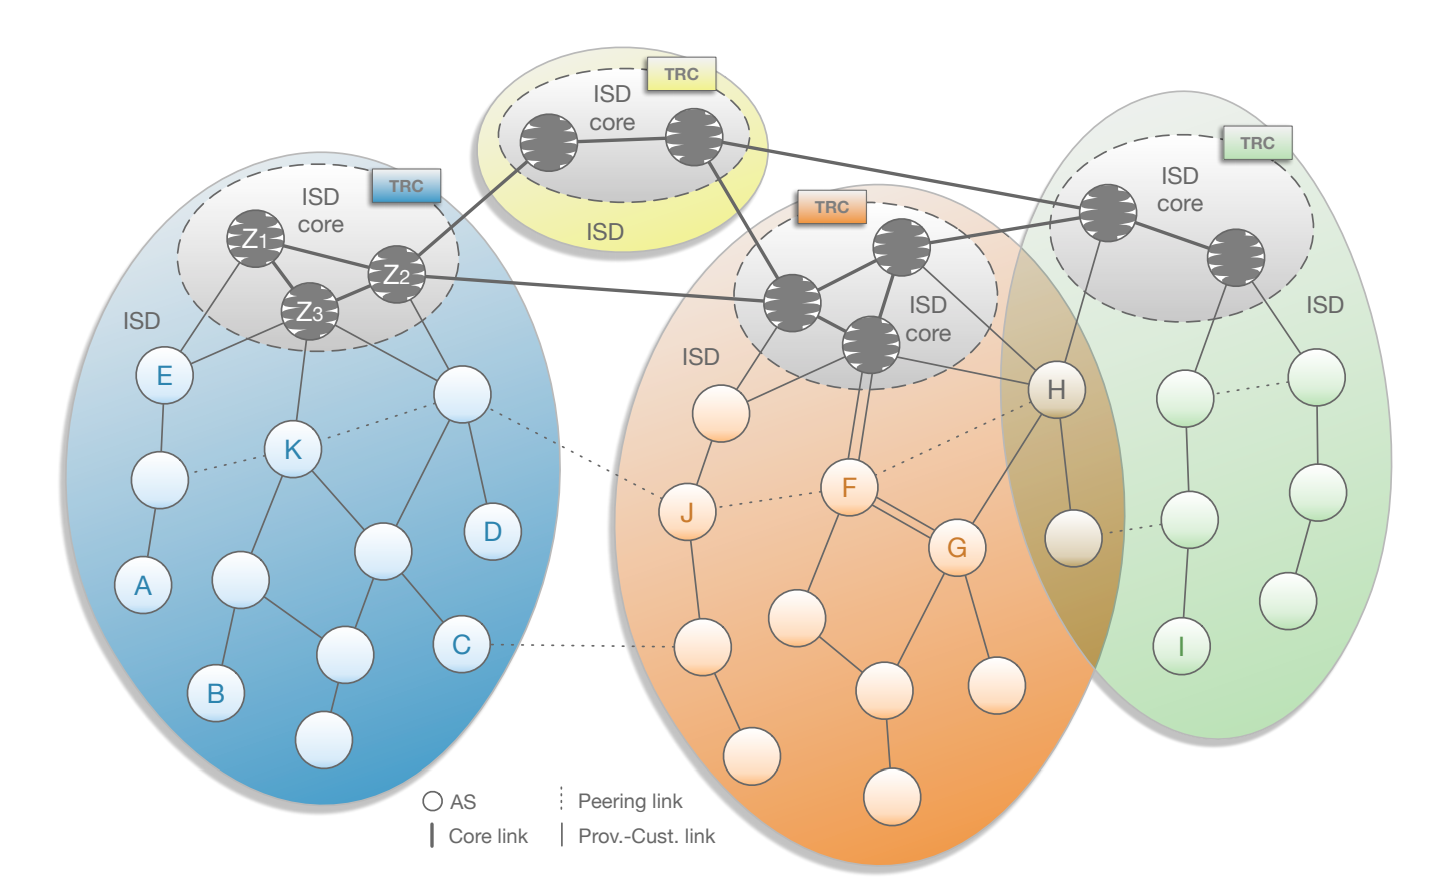
\includegraphics[scale=0.3]{Figures/isd-as.png}}
\decoRule
\caption[ISD-AS representation inside SCION]{Autonomous systems (ASes) grouped into four ISDs. The core
ASes are connected via core links. Non-core ASes are connected
via customer-to-provider or peering links. AS \textit{H} participates in two
ISDs. (Copied from Figure 2.1, Chapter 2 \cite{PeSzReCh2017})}
\label{fig:isd_as}
\end{figure}

\section{Path-Segment Construction in SCION} \label{path_res}
SCION \cite{PeSzReCh2017, scionfwd} uses source-based path selection and embeds the forwarding information inside the packet. To achieve end-to-end communication ASes inside SCION are hierarchically organized to explore the topology and create half-paths. These half-paths are then joined together to form end-to-end AS-levels paths. Once those end-to-end paths are constructed then they can be used for the communication.

\subsection{Topological Structure}
ASes are organized in a tree-based hierarchical structure and the root of the tree are called core ASes and children are called non-core ASes.
\paragraph{Half-Path construction} Each AS has to discover a set of half-paths specifically \textit{up-paths} and \textit{down-paths}. Up-paths represents a set of paths which a non-core AS could use to reach core AS and down-paths are set of paths which a core AS could use to reach non-core ASes.

The ASes then periodically initiates Path-Segment Construction Beacons (PCBs). It contains information about the core AS that initiated the beacon construction and series of AS entries that follows the order of propagation (i.e., each AS appends an entry during beacon propagation). The main purpose of PCB is to explore routing paths. 

\paragraph{Half-Path joining} In SCION end-to-end path can be constructed by joining two half-paths. To be precise source AS combines a one of its up-paths with one of the down-paths to the destination AS. Since every AS can reach the root of the tree and can be reached from root of the tree. Hence there is a guarantee that we can always find a path between a source and a destination AS.

% \subsection{What is beaconing?}
% An ISD core announces a PCB and disseminates it as a policy-constrained multipath flood either within an ISD (to explore intra-ISD paths) or amongst core ASes (to explore inter-ISD paths). This process is referred as beaconing. PCBs accumulate cryptographically protected AS-level path information as they traverse the network. This information is called Hop-Fields (HF) within received PCBs is chained together to create a data transmission path segment that traverses a sequence of ASes. Packet thus contains AS-level path information, which avoid the need for routers to maintain inter-domain forwarding tables. This concept is referred as packet-carried forwarding state (PCFS).

% Not needed put in the end
\section{Addressing Scheme in SCION} \label{addr_scheme}
An ISD-AS number is 64-bits, with the top 16 bits indicating the ISD, and the bottom 48 bits indicating the AS. The text representation uses a "-" separator between the ISD and AS numbers. e.g. 4-ff00:1:f. AS numbering is globally unique, and uses a super-set of the existing BGP AS numbering scheme. The default formatting for AS numbers is very similar to IPv6. It uses a 16-bit ":" separated lower-case hex encoding with leading 0's omitted: 0:0:0 to ffff:ffff:ffff. Note that the :: zero-compression feature of IPv6 is not legal. It has very limited use in a 48-bit address space, and would just add an extra complication for very little gain.

\section{Service Infrastructure} \label{serv_infra}
In order to facilitate control-plane anycast communication, SCION introduces a dedicated service addressing scheme. For instance, a beacon server that wishes to register segments with a remote AS's path service does not have to know the actual address of a remote path server. Instead, the SCION service address of the path service suffices, so that the SCION border router in the remote AS can select an alive instance of the service to deliver the packet to.

\subsection{Beacon Service}
Beacon servers are responsible for generating, receiving, and propagating PCBs to construct path segments, a process that is referred as beaconing. SCION supports two types of beaconing:
\begin{itemize}
    \item Intra-ISD beaconing - Its responsible for constructing path segments from a core AS to non-core ASes within an ISD
    \item Inter-ISD beaconing - Its responsible for constructing path segments amongst core ASes within an ISD and across ISD.
\end{itemize}

\subsection{Path Service}
Path servers store mappings from AS identifiers to set of announced path segments, and are organized as a hierarchical caching system similar to today's DNS. Through beacon servers, ASes select the set of paths segments through which they want to be reached, and upload them to a path server in the ISD core.

\paragraph{Path resolution}
This process allows end hosts to create an end-to-end forwarding path to a destination. It consists of two phases: (a) \textit{path look-up}, where the end host obtains the path segments, and (b) \textit{path combination}, where an actual forwarding path is created from the path segments.

% Trust management inside SCION - TODO
\subsection{Trust Management inside SCION} \label{sec:cert_server}
Certificate servers keep cached copies of TRCs retrieved from the ISD core, keep cached copies of AS certificates, and manage keys and certificates for securing inter-AS communication. Certificate servers are queried by beacon servers when validating the authenticity of PCBs (i.e., when a beacon server lacks a certificate).

\section{SCION Implementation Details} \label{sec:scion_impl}

\subsection{Border Router}
Border routers connect different ASes supporting SCION. The main task of border routers is to forward packets. In the case of a packet containing a service address, the border router forwards it to the appropriate server, and in the case of data packet the border router forwards it either to a host inside the AS or towards the next border router. Since SCION can operate using any communication fabric inside an AS (e.g., OSPF, SDN, MPLS), the internal routers do not need to be changed.

\subsection{Dispatcher}

\subsection{Role of dispatcher}
Currently Linux kernel only understands how to handle IP packets and it does not understand SCION packets. So in order to handle SCION packet on the endhost it needs to act as an overlay over current internet. Dispatcher is that userspace process which receives SCION packet over IP/UDP overlay and handle communication within an AS. As result dispatcher is given a specific UDP port (30041) through which all SCION packets are communicated and define a single process (within each host) that handles all incoming SCION packet.

\paragraph{Implementation details}
The dispatcher performs two tasks: (a) handling encapsulation and decapsulation of the IP/UDP overlay and the SCION Headers, and (b) interacting with the transport protocol stacks. That is dispatcher mediates between applications and transport protocol implementations to process incoming and outgoing packets.

More specifically, for outgoing packets, the QUIC stack and UDP applications send their data along with the packet's metadata. The metadata includes a forwarding path and an address of the first SCION hop (i.e., border router) on the path. The dispatcher, upon receiving the data and its metadata, encapsulates the data and sends the packets to the specified border router. The path and the first-hop address are provided to applications by the SCION daemon which has the required control plane information.

For incoming packets, the dispatcher decapsulates the overlay header and parses the SCION header to identify the transport protocol. The dispatcher processes packets differently for different transport protocol. The dispatcher processes packets differently for different transport protocols. The dispatcher parses the identifier associated with the incoming packet and delivers the packet to the application that is registered for that identifier.

\subsection{SCION Daemon (SCIOND)} \label{background:sciond}
SCIOND is a background process running on endhosts with the goals of
\begin{itemize}
    \item handling SCION control-plane messages, and
    \item providing an API for applications and libraries to interact with SCION control plane.
\end{itemize}
More specifically SCIOND implements the following services
\begin{itemize}
    \item \textbf{Path lookup} Basically SCIOND contacts the local path server on behalf of endhost and caches the results for future use.
    \item \textbf{Topology Information} SCIOND provides information about the topology of the local AS. Topology information includes address of the border routers (with their interface identifiers). Currently it just reads the \texttt{topology.json} to provide that information but in the future there would be a discovery service to help SCIOND to provide that information.
    \item \textbf{Service Address lookup} SCIOND performs service address look ups i.e., converting service address to its overlay IPv4/IPv6 addresses.
    \item \textbf{Trust Management} stores received certificates and TRCs, and checks their authenticity and consistency (when a new certificate/TRC is received). Certificates and TRCs can be provided to application on demand.
\end{itemize}

\subsection{SNET}
\textit{SNET} is the library to write applications based on SCION architecture. It's very similar to golang's \texttt{net} package which is used for writing networking application. SNET provides the following basic APIs:
\begin{itemize}
    \item \texttt{snet.ListenSCION(net string, localAddress snet.Addr) (*Conn, error)} \\
    It's used to start basic SCION server of type depending upon network string such as \texttt{udp} or \texttt{tcp} on the local SCION address specified. It returns a \texttt{Conn} interface if successful or a error string. This interface could be used to read/write packet on the network.
    \item \texttt{snet.DialSCION(net string, laddr, raddr snet.Addr) (*Conn, error)}
    It's used by SCION client to establish a connection with SCION server depending upon network string. This also returns a \texttt{Conn} interface.
\end{itemize}

\subsection{Basic client/server application example}
\inputminted[frame=lines, framesep=2mm, baselinestretch=1.2, fontsize=\footnotesize, linenos]{go}{code_snippets/temp.go}
